\documentclass{standalone}

\usepackage{ifthen}
\usepackage{tikz}
\usetikzlibrary{shapes,arrows,calc,positioning}
\usetikzlibrary{decorations.pathreplacing}


\usepackage{dsfont}
\newcommand{\bra}[1]{\left\langle{#1}\right|}
\newcommand{\ket}[1]{\left|{#1}\right\rangle}
\newcommand{\braket}[2]{\left\langle{#1}|{#1}\right\rangle}
\newcommand{\ketbra}[2]{\left| #1 \right\rangle \left\langle#2\right|}
\newcommand{\Id}{\mathds{I}}

\newsavebox{\measure}
\savebox{\measure}{%
    
\begin{tikzpicture}[scale=0.65]
        \draw[thin, black] (0.2,0.1) --(0.4,0.6);
%        \draw (-0.25,0.2) -- (0.5,0.2);
        \draw[thin] plot [smooth,tension=1.2] coordinates{(-0.2,0.2) (0.2,0.35) (0.6,0.2)};
%        \node[] at (-0.2,0.4) {\tiny{0}};
%        \node[] at (0.6,0.4) {\tiny{1}};
    \end{tikzpicture}%
}

\begin{document}

% We need layers to draw the block diagram
%\pgfdeclarelayer{background}
%\pgfdeclarelayer{foreground}
%\pgfsetlayers{background,main,foreground}

%\newcommand{\ket}[1]{\left|{#1}\right\rangle}

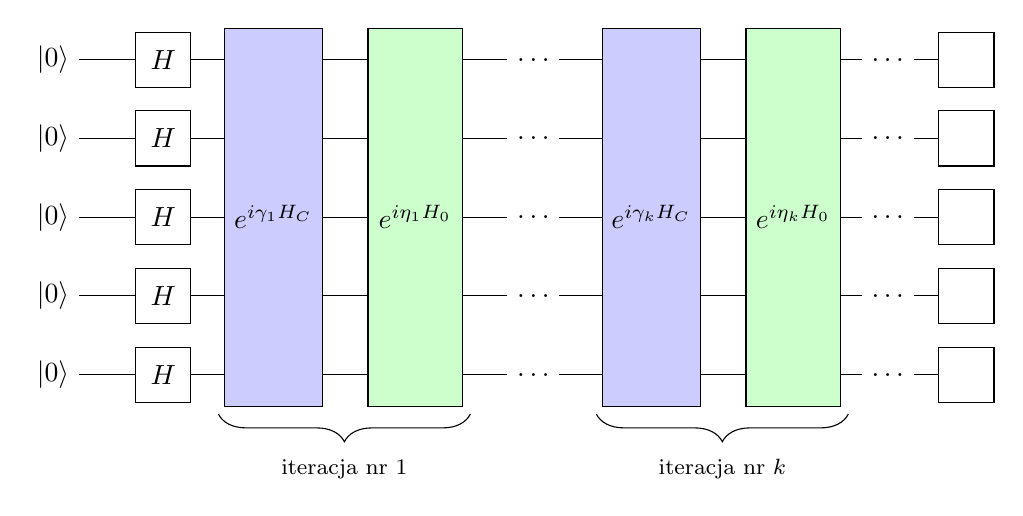
\begin{tikzpicture}

  \tikzstyle{op1q} = [draw,fill=white,minimum size=0.7cm]
  \tikzstyle{measure} = [draw,fill=white,minimum size=0.7cm]
  \tikzstyle{op2qC} = [draw,fill=blue!20,minimum height=4.8cm, minimum width=1.2cm]
  \tikzstyle{op2qM} = [draw,fill=green!20,minimum height=4.8cm, minimum width=1.2cm]


  \foreach \x in {0,...,4} {

    \node at (-0.4,\x) (q\x) {$\ket{0}$};
    \node[op1q] (opH1\x) at (1,\x) {$H$} edge [-] (q\x);
    \node[] (wire1\x{}dots) at (5.7,\x) {$\dots$} edge [-] (opH1\x);
    \node[] (wire2\x{}dots) at (10.2,\x) {$\dots$} edge [-] (wire1\x{}dots);
    \node[measure] (measure\x) at (11.2,\x) {\usebox{\measure}} edge [-] (wire2\x{}dots);
}

%  \node[measure] (measure) at (6.8,0) {\usebox{\measure}} edge [-] (wire0dots);
%  \node[measure] (measure) at (6.8,1) {\usebox{\measure}} edge [-] (wire1dots);
%  \node[measure] (measure) at (6.8,2) {\usebox{\measure}} edge [-] (wire2dots);
%  \node[measure] (measure) at (6.8,3) {\usebox{\measure}} edge [-] (wire3dots);
%
  \node[op2qC] (opHH) at (2.4,2.0) {$e^{i\gamma_1 H_C}$};
  \node[op2qM] (opHH) at (4.2,2.0) {$e^{i\eta_1 H_0}$};

  \node[op2qC] (opHH) at (7.2,2.0) {$e^{i\gamma_k H_C}$};
  \node[op2qM] (opHH) at (9.0,2.0) {$e^{i\eta_k H_0}$};


%  \node[] at (5,-1) {iteracja wykonywana $O(\sqrt{N})$ razy};

  \draw [decorate,decoration={brace,amplitude=10pt}] (4.9,-0.5) -- (1.7,-0.5) node [black,midway,yshift=-0.7cm] {\footnotesize{iteracja nr 1}};

  \draw [decorate,decoration={brace,amplitude=10pt}] (9.7,-0.5) -- (6.5,-0.5) node [black,midway,yshift=-0.7cm] {\footnotesize{iteracja nr $k$}};




\end{tikzpicture}

\end{document}